%----------------------- Wydruk dwustronny ---------------
%\documentclass[12pt,twoside,a4paper]{book} % 
%----------------------- Wydruk jednostronny ---------------
\documentclass[12pt,oneside,a4paper]{book} % jednostronnego

\usepackage{polski}
\usepackage[utf8]{inputenc} %opcja dla edytorów kodujących polskie znaki w utf8
%\usepackage[cp1250]{inputenc} %opcja dla edytorów kodujących polskie znaki w windows-1250
\usepackage{lmodern}
\usepackage{indentfirst}
\usepackage[protrusion=false]{microtype}
\DisableLigatures{encoding = *, family = * }
\usepackage{fancyhdr}
\usepackage{pstricks,graphicx}
\usepackage{amssymb}
\usepackage{float}

\usepackage{pdflscape}
\usepackage{diagbox}

%---------------Zbiory liczbowe
\newcommand{\R}{\mathbb{R}}
\newcommand{\N}{\mathbb{N}}
\newcommand{\K}{\mathbb{K}}
\newcommand{\C}{\mathcal{C}}
\newcommand{\p}{\mathcal{P}}
%------------kwantyfikatory--------------
\newcommand{\fal}{\mbox{{\Large $\forall\,$}}}
\newcommand{\ext}{\mbox{{\Large $\exists\,$}}}
%------------------definicje środowisk-----------------
\usepackage{theorem}
\theoremstyle{break}
\theorembodyfont{\it}
\newtheorem{twr}{Twierdzenie}[chapter]
\newtheorem{lem}{Lemat}[chapter]
\theorembodyfont{\rm}
\newtheorem{defi}{Definicja}[chapter]
\newtheorem{wni}{Wniosek}[chapter]
\newtheorem{prz}{Przykład}[chapter]
\newenvironment{dowod}{\par\vspace{0.1cm}\par{ \sc Dowód.}}{\hfill $\blacksquare$\par\vspace{0.4cm}\par}
% ----------ustawienia wymiarow strony
\usepackage{geometry}

\newgeometry{tmargin=2.5cm, bmargin=2.5cm, headheight=14.5pt, inner=3cm, outer=2.5cm} 

\linespread{1.1} %-zmiana interlinii


\fancypagestyle{mylandscape}{
\fancyhf{} %Clears the header/footer
\fancyfoot{% Footer
\makebox[\textwidth][r]{% Right
  \rlap{\hspace{.75cm}% Push out of margin by \footskip
    \smash{% Remove vertical height
      \raisebox{4.87in}{% Raise vertically
        \rotatebox{90}{\thepage}}}}}}% Rotate counter-clockwise
\renewcommand{\headrulewidth}{0pt}% No header rule
\renewcommand{\footrulewidth}{0pt}% No footer rule
}

%---------------- Normalne środowiska --------------------
\usepackage{amsmath}

%----------nagłowki i żywa pagina ------------
\pagestyle{fancy} 
%--------------- Wydruk dwustronny
%\cfoot[]{} 
%\lhead[{\scriptsize{\it \thepage}}]{}
%\chead[{\scriptsize\leftmark}]{{\scriptsize \rightmark}}
%\rhead[]{{\scriptsize{\it \thepage}}}
%--------------- Wydruk jednostronny
\fancyhead[C]{} 
\fancyfoot[C]{\thepage}
\fancyhead[L]{\scriptsize\leftmark}
\fancyhead[R]{\scriptsize\rightmark}

\renewcommand{\chaptermark}[1]{%
\markboth{\MakeUppercase{%
\chaptername}\ \thechapter.%
\ #1}{}}

\usepackage[most]{tcolorbox}
\let\includegraphicsold\includegraphics
\newcommand{\includegraphicsborder}[2][]{\tcbox{\includegraphicsold[#1]{#2}}}

\renewcommand{\sectionmark}[1]{\markright{\thesection.\ #1}}

\usepackage[hidelinks]{hyperref}

\usepackage{graphics}
\graphicspath{ {images/} }

\usepackage{listings}

\renewcommand{\lstlistlistingname}{Spis listingów}
\renewcommand{\lstlistingname}{Listing}

\lstset{
  basicstyle=\footnotesize,
  numbers=left,
  mathescape=true
}

\usepackage{booktabs}

\newcommand\tabularhead[2]{
  \begin{table}[ht]
    \label{#2}
    \caption{#1}
    \begin{tabular}{|p{0.35\linewidth}|p{0.6\linewidth}|}
    \hline
    \textbf{#1}\\
    \hline
}
\newcommand\addrow[2]{#1 &#2\\ \hline}

\newcommand\addmulrow[2]{ \begin{minipage}[t][][t]{2.5cm}#1\end{minipage}
   &\begin{minipage}[t][][t]{8cm}
    \begin{enumerate} #2   \end{enumerate}
    \end{minipage}\\ }

\newenvironment{usecase}{\tabularhead}
{\hline\end{tabular}\end{table}}



%-----------------właściwa część pracy-----------------
\begin{document}
\thispagestyle{empty}
\begin{center}
  \Large
  \bf{UNIWERSYTET ŚLĄSKI}\\
  \bf{\sf{WYDZIAŁ NAUK ŚCISŁYCH I TECHNICZNYCH}}\\[25mm]
  \large


  Sprawozdanie\\
  z przedmiotu\\
  tyfloinformatyka\\[25mm]
\end{center}
\begin{flushright}
  \large
  Autorzy:\\
  Kacper Małachowski\\
\end{flushright}
\vspace*{\fill}
\begin{center}
  Informatyka II Stopnia\\
  Lato 2023/2024\\
  I rok, grupa 3\\[25mm]
\end{center}

\chapter*{Lupa}

Użycie programu powiększajacego.

\begin{figure}[H]
  \centering
  
\includegraphics[width=1\textwidth]{magnifier.png}
\end{figure}

\chapter*{Narrator}

Użycie programu udźwiękawiajacego.

\begin{figure}[H]
  \centering
  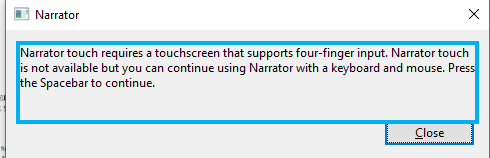
\includegraphics[width=1\textwidth]{narrator.png}
\end{figure}

\chapter*{NVDA}

Uruchomienie programu NVDA.

\begin{figure}[H]
  \centering
  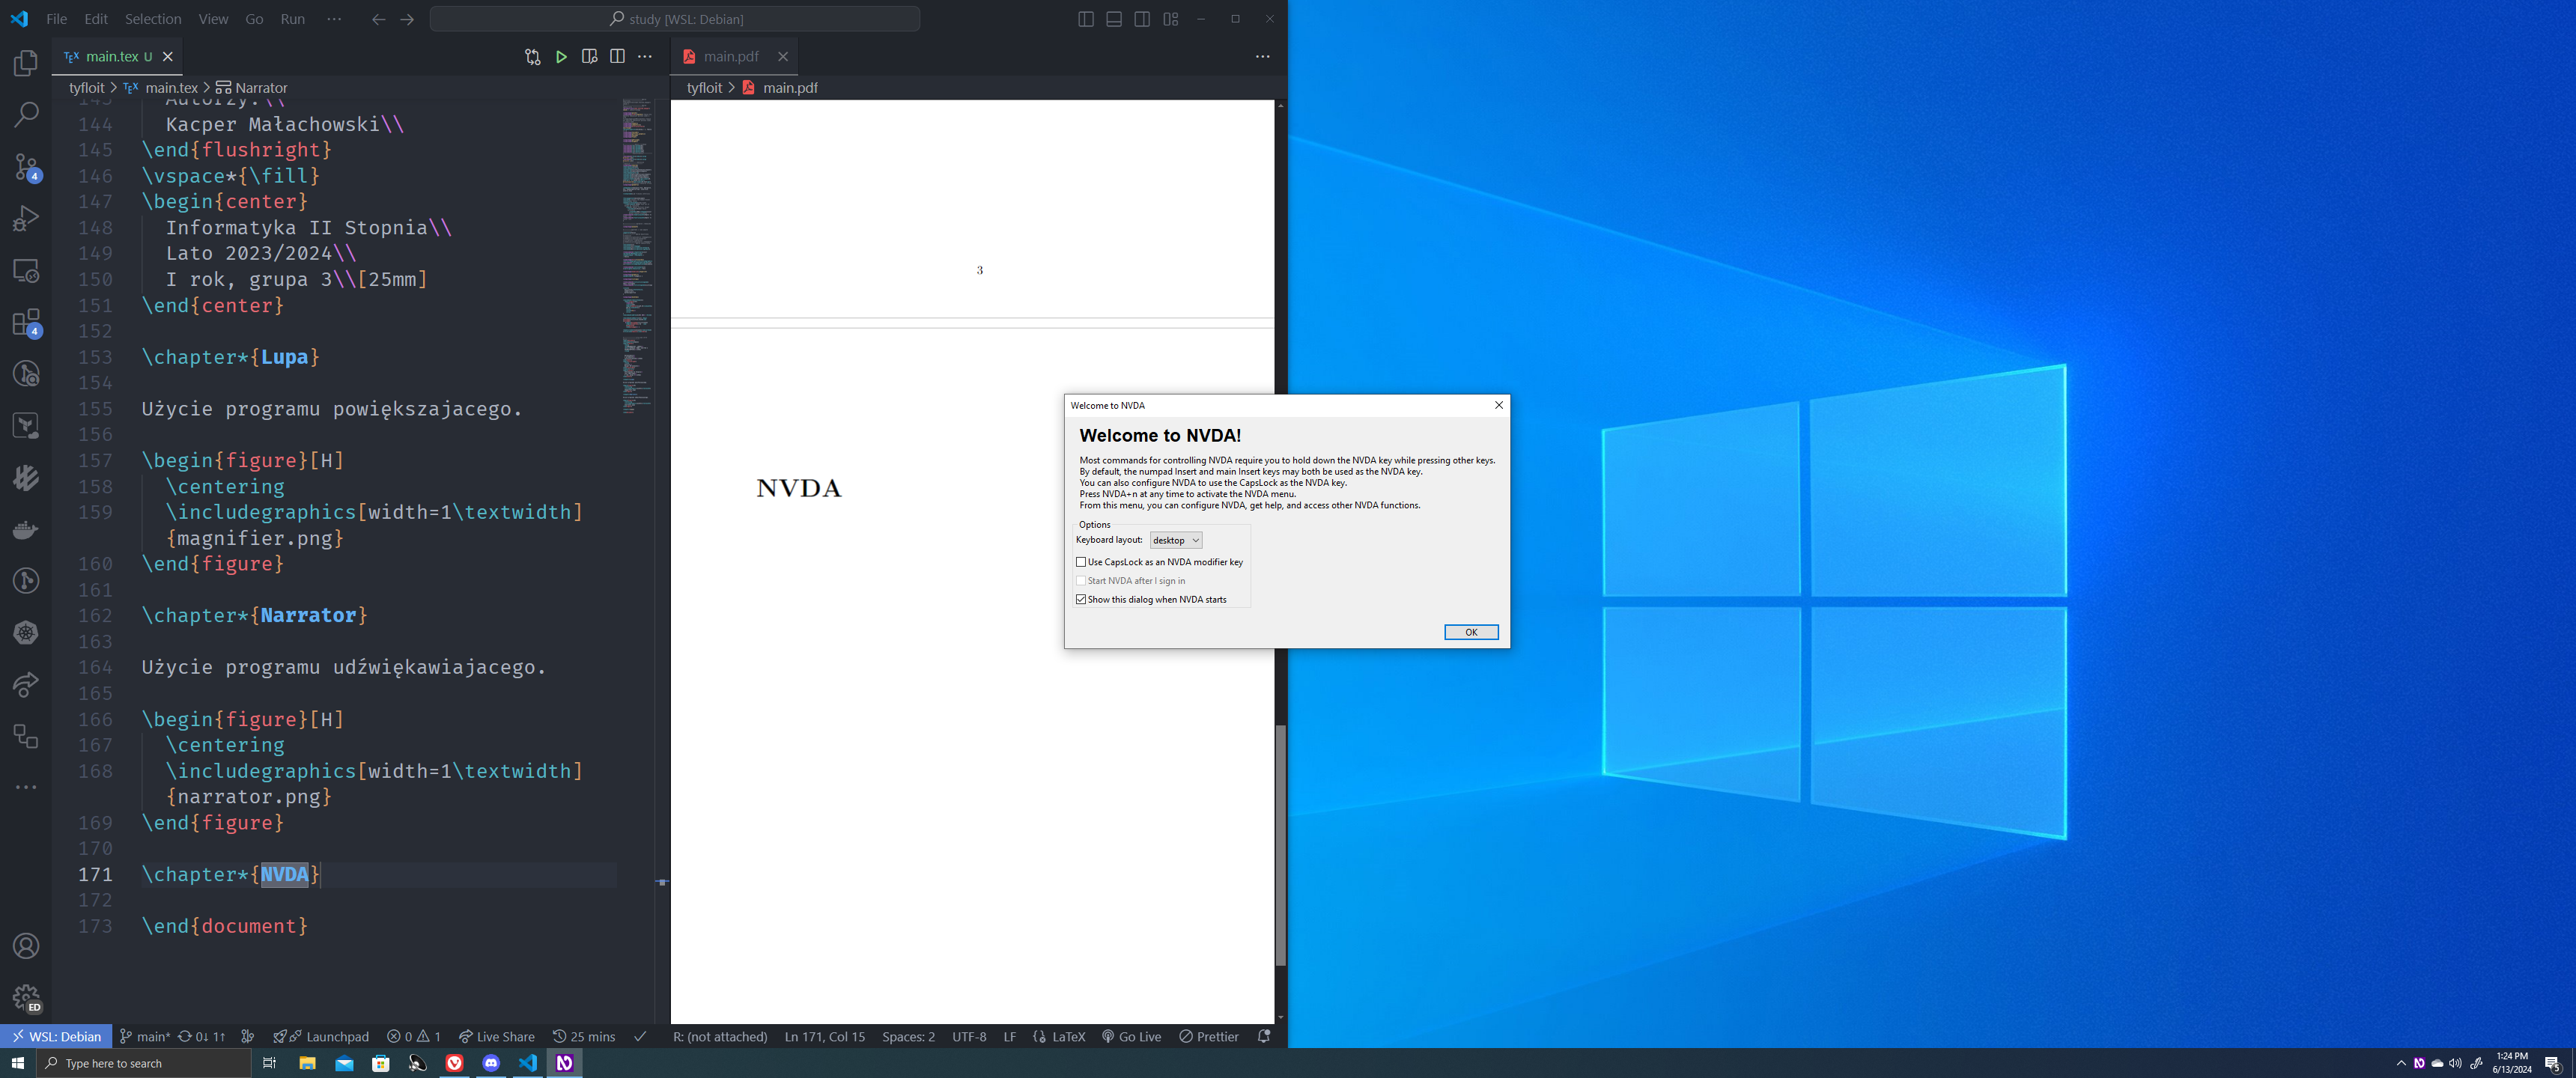
\includegraphics[width=1\textwidth]{nvda.png}
\end{figure}

Opcje programu NVDA.

\begin{figure}[H]
  \centering
  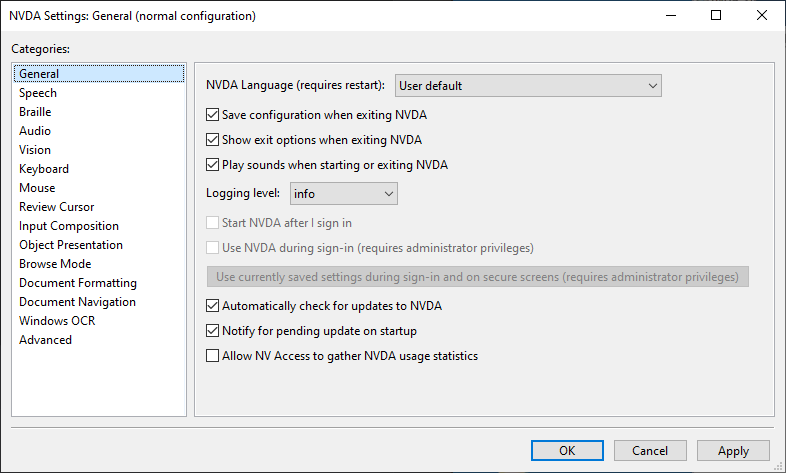
\includegraphics[width=1\textwidth]{nvda-settings.png}
\end{figure}

\chapter*{Opis strony Paffsair.pl}

Niski kontrast tekstu.
\begin{figure}[H]
  \centering
  
\includegraphics[width=1\textwidth]{paffsair/low-contrast.png}
\end{figure}

Tekst alternatywny kiepsko opisujacy obrazek przycisku prowadzącego do YT.

\begin{figure}[H]
  \centering
  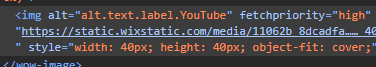
\includegraphics[width=1\textwidth]{paffsair/not-meaningfull-alt.png}
\end{figure}

Tekst alternatywny jako nazwa pliku.

\begin{figure}[H]
  \centering
  
\includegraphics[width=1\textwidth]{paffsair/alt-text-as-filename.png}
\end{figure}
\newpage
Menu to znaczniki p.
\begin{figure}[H]
  \centering
  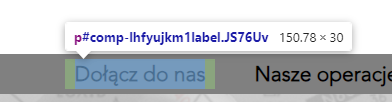
\includegraphics[width=1\textwidth]{paffsair/link-as-p.png}
\end{figure}

Klikalny element zrealizowany znacnzikiem span.
\begin{figure}[H]
  \centering
  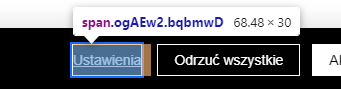
\includegraphics[width=1\textwidth]{paffsair/clickable-span.png}
\end{figure}

Brak znacznika h1.

Menu jest niewybieralne poprzez Tab z powodu zastowania błednych znaczników.

Zdublowane linki, zwiększające ilość powtórzeń dla czytników ekranu.
\begin{figure}[H]
  \centering
  
\includegraphics[width=1\textwidth]{paffsair/reduntant-links.png}
\end{figure}

Tekst widoczny tylko dla czytników ekranu.
\begin{figure}[H]
  \centering
  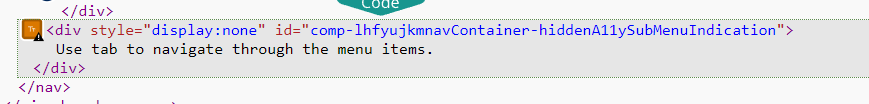
\includegraphics[width=1\textwidth]{paffsair/text-hidden.png}
\end{figure}

\end{document}